\chapter{Generative models for discrete data}

\section{Generative classifier}
\begin{equation}\label{eqn:Generative-classifier}
p(y=c|\vec{x},\vec{\theta})=\dfrac{p(y=c|\vec{\theta})p(\vec{x}|y=c,\vec{\theta})}{\sum_{c'}{p(y=c'|\vec{\theta})p(\vec{x}|y=c',\vec{\theta})}}
\end{equation}

This is called a \textbf{generative classifier}, since it specifies how to generate the data using the \textbf{class conditional density} $p(\vec{x}|y=c)$ and the class prior $p(y=c)$. An alternative approach is to directly fit the class posterior, $p(y=c|\vec{x})$ ;this is known as a \textbf{discriminative classifier}. 


\section{Bayesian concept learning}
Psychological research has shown that people can learn concepts from positive examples alone (Xu and Tenenbaum 2007).

We can think of learning the meaning of a word as equivalent to \textbf{concept learning}, which in turn is equivalent to binary classification. To see this, define $f(\vec{x})=1$ if x is an example of the concept $C$, and $f(\vec{x})=0$ otherwise. Then the goal is to learn the indicator function $f$, which just defines which elements are in the set $C$.


\subsection{Likelihood}
\begin{equation}
p(\mathcal{D}|h) \triangleq \left(\dfrac{1}{\text{size}(h)}\right)^N=\left(\dfrac{1}{|h|}\right)^N
\end{equation}

This crucial equation embodies what Tenenbaum calls the \textbf{size principle}, which means the model favours the simplest (smallest) hypothesis consistent with the data. This is more commonly known as \textbf{Occam’s razor}\footnote{\url{http://en.wikipedia.org/wiki/Occam\%27s_razor}}.


\subsection{Prior}
The prior is decided by human, not machines, so it is subjective. The subjectivity of the prior is controversial. For example, that a child and a math professor will reach different answers. In fact, they presumably not only have different priors, but also different hypothesis spaces. However, we can finesse that by defining the hypothesis space of the child and the math professor to be the same, and then setting the child’s prior weight to be zero on certain “advanced” concepts. Thus there is no sharp distinction between the prior and the hypothesis space.

However, the prior is the mechanism by which background knowledge can be brought to bear on a problem. Without this, rapid learning (i.e., from small samples sizes) is impossible.


\subsection{Posterior}
The posterior is simply the likelihood times the prior, normalized.
\begin{equation}
p(h|\mathcal{D}) \triangleq \dfrac{p(\mathcal{D}|h)p(h)}{\sum_{h' \in \mathcal{H}}p(\mathcal{D}|h')p(h')}=\dfrac{\mathbb{I}(\mathcal{D} \in h)p(h)}{\sum_{h' \in \mathcal{H}}\mathbb{I}(\mathcal{D} \in h')p(h')}
\end{equation}
where $\mathbb{I}(\mathcal{D} \in h)p(h)$ is 1 \textbf{iff}(iff and only if) all the data are in the extension of the hypothesis $h$.

In general, when we have enough data, the posterior $p(h|\mathcal{D})$ becomes peaked on a single concept, namely the MAP estimate, i.e.,
\begin{equation}
p(h|\mathcal{D}) \rightarrow \hat{h}^{MAP}
\end{equation}
where $\hat{h}^{MAP}$ is the posterior mode,
\begin{equation}\begin{split}
\hat{h}^{MAP} & \triangleq \arg\max\limits_h p(h|\mathcal{D})=\arg\max\limits_h p(\mathcal{D}|h)p(h) \\
    & =\arg\max\limits_h [\log p(\mathcal{D}|h) + \log p(h)]
\end{split}\end{equation}

Since the likelihood term depends exponentially on $N$, and the prior stays constant, as we get more and more data, the MAP estimate converges towards the \textbf{maximum likelihood estimate} or \textbf{MLE}:
\begin{equation}
\hat{h}^{MLE} \triangleq \arg\max\limits_h p(\mathcal{D}|h)=\arg\max\limits_h \log p(\mathcal{D}|h)
\end{equation}

In other words, if we have enough data, we see that the \textbf{data overwhelms the prior}.


\subsection{Posterior predictive distribution}
The concept of \textbf{posterior predictive distribution}\footnote{\url{http://en.wikipedia.org/wiki/Posterior_predictive_distribution}} is normally used in a Bayesian context, where it makes use of the entire posterior distribution of the parameters given the observed data to yield a probability distribution over an interval rather than simply a point estimate. 
\begin{equation}
p(\tilde{\vec{x}}|\mathcal{D}) \triangleq \mathbb{E}_{h|\mathcal{D}}[p(\tilde{\vec{x}}|h)] = \begin{cases}
\sum_h p(\tilde{\vec{x}}|h)p(h|\mathcal{D}) \\
\int p(\tilde{\vec{x}}|h)p(h|\mathcal{D})\mathrm{d}h
\end{cases}
\end{equation}

This is just a weighted average of the predictions of each individual hypothesis and is called \textbf{Bayes model averaging}(Hoeting et al. 1999). 


\section{The beta-binomial model}


\subsection{Likelihood}
Given $X \sim \text{Bin}(\theta)$, the likelihood of $\mathcal{D}$ is given by
\begin{equation}
p(\mathcal{D}|\theta)= \text{Bin}(N_1|N,\theta)
\end{equation}


\subsection{Prior}
\begin{equation}
\text{Beta}(\theta|a,b) \propto \theta^{a-1}(1-\theta)^{b-1}
\end{equation}

The parameters of the prior are called \textbf{hyper-parameters}.


\subsection{Posterior}
\begin{equation}\begin{split}\label{eqn:beta-binomial-posterior}
p(\theta|\mathcal{D}) & \propto \text{Bin}(N_1|N_1+N_0,\theta)\text{Beta}(\theta|a,b) \\
    & =\text{Beta}(\theta|N_1+a,N_0b)
\end{split}\end{equation}

Note that updating the posterior sequentially is equivalent to updating in a single batch. To see this, suppose we have two data sets $\mathcal{D}_a$ and $\mathcal{D}_b$ with sufficient statistics $N_1^a,N_0^a$ and $N_1^b,N_0^b$. Let $N_1=N_1^a+N_1^b$ and $N_0=N_0^a+N_0^b$ be the sufficient statistics of the combined datasets. In batch mode we have
\begin{align*}
p(\theta|\mathcal{D}_a,\mathcal{D}_b)& = p(\theta,\mathcal{D}_b|\mathcal{D}_a)p(\mathcal{D}_a) \\
               &\propto p(\theta,\mathcal{D}_b|\mathcal{D}_a) \\
               & = p(\mathcal{D}_b,\theta|\mathcal{D}_a) \\
			   & = p(\mathcal{D}_b|\theta)p(\theta|\mathcal{D}_a) \\
			   & \text{Combine Equation \ref{eqn:beta-binomial-posterior} and \ref{eqn:binomial-pmf}} \\
			   & =\text{Bin}(N_1^b|\theta, N_1^b+N_0^b)\text{Beta}(\theta|N_1^a+a,N_0^a+b) \\
			   & =\text{Beta}(\theta|N_1^a+N_1^b+a,N_0^a+N_0^b+b)
\end{align*}

This makes Bayesian inference particularly well-suited to \textbf{online learning}, as we will see later.

\subsubsection{Posterior mean and mode}
\label{sec:beta-binomial-Posterior-mean-and-mode}
From Table \ref{tab:beta-distribution}, the posterior mean is given by
\begin{equation}
\bar{\theta}=\dfrac{a+N_1}{a+b+N}
\end{equation}

The mode is given by
\begin{equation}
\hat{\theta}_{MAP}=\dfrac{a+N_1-1}{a+b+N-2}
\end{equation}

If we use a uniform prior, then the MAP estimate reduces to the MLE,
\begin{equation}
\hat{\theta}_{MLE}=\dfrac{N_1}{N}
\end{equation}

We will now show that the posterior mean is convex combination of the prior mean and the MLE, which captures the notion that the posterior is a compromise between what we previously believed and what the data is telling us.

\subsubsection{Posterior variance}
The mean and mode are point estimates, but it is useful to know how much we can trust them. The variance of the posterior is one way to measure this. The variance of the Beta posterior is given by
\begin{equation}
\text{var}(\theta|\mathcal{D})=\dfrac{(a+N_1)(b+N_0)}{(a+N_1+b+N_0)^2(a+N_1+b+N_0+1)}
\end{equation}

We can simplify this formidable expression in the case that $N \gg a, b$, to get
\begin{equation}
\text{var}(\theta|\mathcal{D}) \approx \dfrac{N_1N_0}{NNN}=\dfrac{\hat{\theta}_{MLE}(1-\hat{\theta}_{MLE})}{N}
\end{equation}


\subsection{Posterior predictive distribution}
So far, we have been focusing on inference of the unknown parameter(s). Let us now turn our attention to prediction of future observable data.

Consider predicting the probability of heads in a single future trial under a Beta$(a, b)$posterior. We have
\begin{align}
p(\tilde{x}|\mathcal{D})& =\int_0^1 p(\tilde{x}|\theta)p(\theta|\mathcal{D})\mathrm{d}\theta \nonumber \\
                        & =\int_0^1 \theta\text{Beta}(\theta|a,b)\mathrm{d}\theta \nonumber \\
						& =\mathbb{E}[\theta|\mathcal{D}]=\dfrac{a}{a+b}
\end{align}

\subsubsection{Overfitting and the black swan paradox}
Let us now derive a simple Bayesian solution to the problem. We will use a uniform prior, so $a=b=1$. In this case, plugging in the posterior mean gives \textbf{Laplace’s rule of succession}
\begin{equation}
p(\tilde{x}|\mathcal{D})=\dfrac{N_1+1}{N_0+N_1+1}
\end{equation}

This justifies the common practice of adding 1 to the empirical counts, normalizing and then plugging them in, a technique known as \textbf{add-one smoothing}. (Note that plugging in the MAP parameters would not have this smoothing effect, since the mode becomes the MLE if $a=b=1$, see Section \ref{sec:beta-binomial-Posterior-mean-and-mode}.)

\subsubsection{Predicting the outcome of multiple future trials}
Suppose now we were interested in predicting the number of heads, $\tilde{x}$, in $M$ future trials. This is given by
\begin{align}
p(\tilde{x}|\mathcal{D})& =\int_0^1 \text{Bin}(\tilde{x}|M,\theta)\text{Beta}(\theta|a,b)\mathrm{d}\theta \\
                        & =\dbinom{M}{\tilde{x}}\dfrac{1}{B(a,b)}\int_0^1 \theta^{\tilde{x}}(1-\theta)^{M-\tilde{x}}\theta^{a-1}(1-\theta)^{b-1}\mathrm{d}\theta
\end{align}

We recognize the integral as the normalization constant for a Beta$(a+\tilde{x}, M−\tilde{x}+b)$ distribution. Hence
\begin{equation}
\int_0^1 \theta^{\tilde{x}}(1-\theta)^{M-\tilde{x}}\theta^{a-1}(1-\theta)^{b-1}\mathrm{d}\theta=B(\tilde{x}+a,M-\tilde{x}+b)
\end{equation}

Thus we find that the posterior predictive is given by the following, known as the (compound) \textbf{beta-binomial distribution}:
\begin{equation}
Bb(x|a,b,M) \triangleq \dbinom{M}{x}\dfrac{B(x+a,M-x+b)}{B(a,b)}
\end{equation}

This distribution has the following mean and variance
\begin{equation}
\text{mean}=M\dfrac{a}{a+b} \text{ , var}=\dfrac{Mab}{(a+b)^2}\dfrac{a+b+M}{a+b+1}
\end{equation}

This process is illustrated in Figure \ref{fig:beta-binomial-distribution}. We start with a Beta$(2,2)$ prior, and plot the posterior predictive density after seeing $N_1 =3$ heads and $N_0 =17$ tails. Figure \ref{fig:beta-binomial-distribution}(b) plots a plug-in approximation using a MAP estimate. We see that the Bayesian prediction has longer tails, spreading its probability mass more widely, and is therefore less prone to overfitting and blackswan type paradoxes.

\begin{figure}[hbtp]
\centering
\subfloat[]{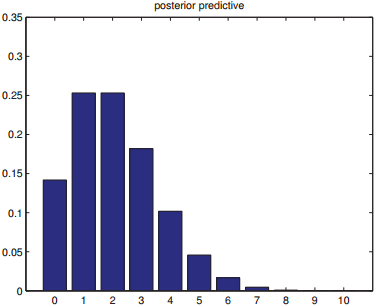
\includegraphics[scale=.60]{beta-binomial-distribution-a.png}} \\
\subfloat[]{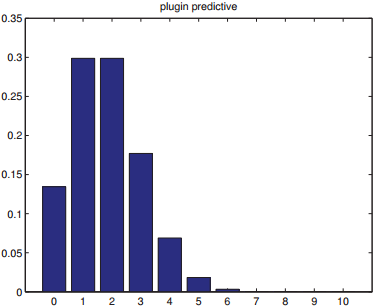
\includegraphics[scale=.60]{beta-binomial-distribution-b.png}}
\caption{(a) Posterior predictive distributions after seeing $N_1=3,N_0=17$. (b) MAP estimation.}
\label{fig:beta-binomial-distribution} 
\end{figure}


\section{The Dirichlet-multinomial model}
In the previous section, we discussed how to infer the probability that a coin comes up heads. In this section, we generalize these results to infer the probability that a dice with $K$ sides comes up as face $k$. 


\subsection{Likelihood}
Suppose we observe $N$ dice rolls, $\mathcal{D}=\{x_1,x_2,\cdots,x_N\}$, where $x_i \in \{1,2,\cdots,K\}$. The likelihood has the form
\begin{equation}
p(\mathcal{D}|\vec{\theta}) = \dbinom{N}{N_1 \cdots N_k} \prod\limits_{k=1}^K\theta_k^{N_k} \quad \text{where } N_k=\sum\limits_{i=1}^N \mathbb{I}(y_i=k)
\end{equation}
almost the same as Equation \ref{eqn:multinomial-pmf}.


\subsection{Prior}
\begin{equation}
\text{Dir}(\vec{\theta}|\vec{\alpha}) = \dfrac{1}{B(\vec{\alpha})}\prod\limits_{k=1}^K \theta_k^{\alpha_k-1}\mathbb{I}(\vec{\theta} \in S_K)
\end{equation}


\subsection{Posterior}
\begin{align}
p(\vec{\theta}|\mathcal{D})& \propto p(\mathcal{D}|\vec{\theta})p(\vec{\theta}) \\
     & \propto \prod\limits_{k=1}^K\theta_k^{N_k}\theta_k^{\alpha_k-1} = \prod\limits_{k=1}^K\theta_k^{N_k+\alpha_k-1}\\
	 & =\text{Dir}(\vec{\theta}|\alpha_1+N_1,\cdots,\alpha_K+N_K)
\end{align}

From Equation \ref{eqn:Dirichlet-properties}, the MAP estimate is given by
\begin{equation}\label{eqn:Dir-MAP}
\hat{\theta}_k=\dfrac{N_k+\alpha_k-1}{N+\alpha_0-K}
\end{equation}

If we use a uniform prior, $\alpha_k=1$, we recover the MLE:
\begin{equation}\label{eqn:Dirichlet-multinomial-posterior-MLE}
\hat{\theta}_k=\dfrac{N_k}{N}
\end{equation}


\subsection{Posterior predictive distribution}
The posterior predictive distribution for a single multinoulli trial is given by the following expression:
\begin{align}
p(X=j|\mathcal{D})& =\int p(X=j|\vec{\theta})p(\vec{\theta}|\mathcal{D})\mathrm{d}\vec{\theta} \\
    & =\int p(X=j|\theta_j)\left[\int p(\vec{\theta}_{-j}, \theta_j|\mathcal{D})\mathrm{d}\vec{\theta}_{-j}\right]\mathrm{d}\theta_j \\
	& =\int \theta_jp(\theta_j|\mathcal{D})\mathrm{d}\theta_j=\mathbb{E}[\theta_j|\mathcal{D}]=\dfrac{\alpha_j+N_j}{\alpha_0+N}
\end{align}
where $\vec{\theta}_{-j}$ are all the components of \vec{\theta} except $\theta_j$.

The above expression avoids the zero-count problem. In fact, this form of Bayesian smoothing is even more important in the multinomial case than the binary case, since the likelihood of data sparsity increases once we start partitioning the data into many categories.


\section{Naive Bayes classifiers}
\label{sec:NBC}
Assume the features are \textbf{conditionally independent} given the class label, then the class conditional density has the following form
\begin{equation}
p(\vec{x}|y=c,\vec{\theta})=\prod\limits_{j=1}^D p(x_j|y=c,\vec{\theta}_{jc})
\end{equation}

The resulting model is called a \textbf{naive Bayes classifier}(NBC).

The form of the class-conditional density depends on the type of each feature. We give some possibilities below:
\begin{itemize}
\item{In the case of real-valued features, we can use the Gaussian distribution: $p(\vec{x}|y,\vec{\theta})=\prod_{j=1}^D \mathcal{N}(x_j|\mu_{jc},\sigma_{jc}^2)$, where $\mu_{jc}$ is the mean of feature $j$ in objects of class $c$, and $\sigma_{jc}^2$ is its variance.}
\item{In the case of binary features, $x_j \in \{0,1\}$, we can use the Bernoulli distribution: $p(\vec{x}|y,\vec{\theta})=\prod_{j=1}^D \text{Ber}(x_j|\mu_{jc})$, where $\mu_{jc}$ is the probability that feature $j$ occurs in class $c$. This is sometimes called the \textbf{multivariate Bernoulli naive Bayes} model. We will see an application of this below.}
\item{In the case of categorical features, $x_j \in \{a_{j1},a_{j2},\cdots, a_{jS_j}\}$, we can use the multinoulli distribution: $p(\vec{x}|y,\vec{\theta})=\prod_{j=1}^D \text{Cat}(x_j|\vec{\mu}_{jc})$, where $\vec{\mu}_{jc}$ is a histogram over the $K$ possible values for $x_j$ in class $c$.}
\end{itemize}

Obviously we can handle other kinds of features, or use different distributional assumptions. Also, it is easy to mix and match features of different types.


\subsection{Optimization}
\label{sec:NBC-Optimization}
We now discuss how to “train” a naive Bayes classifier. This usually means computing the MLE or the MAP estimate for the parameters. However, we will also discuss how to compute the full posterior, $p(\vec{\theta}|\mathcal{D})$.

\subsubsection{MLE for NBC}
The probability for a single data case is given by
\begin{equation}\begin{split}
p(\vec{x}_i,y_i|\vec{\theta}) & =p(y_i|\vec{\pi})\prod\limits_j p(x_{ij}|\vec{\theta}_j) \\
  & =\prod\limits_c \pi_c^{\mathbb{I}(y_i=c)} \prod\limits_j\prod\limits_c p(x_{ij}|\vec{\theta}_{jc})^{\mathbb{I}(y_i=c)}
\end{split}\end{equation}

Hence the log-likelihood is given by
\begin{equation}
p(\mathcal{D}|\vec{\theta})=\sum\limits_{c=1}^C{N_c\log\pi_c}+ \sum\limits_{j=1}^D{\sum\limits_{c=1}^C{\sum\limits_{i:y_i=c}{\log p(x_{ij}|\vec{\theta}_{jc})}}}
\end{equation}
where $N_c \triangleq \sum\limits_i \mathbb{I}(y_i=c)$ is the number of feature vectors in class $c$.

We see that this expression decomposes into a series of terms, one concerning $\vec{\pi}$, and $DC$ terms containing the $\theta_{jc}$’s. Hence we can optimize all these parameters separately.

From Equation \ref{eqn:Dirichlet-multinomial-posterior-MLE}, the MLE for the class prior is given by
\begin{equation}
\hat{\pi}_c=\dfrac{N_c}{N}
\end{equation}

The MLE for $\theta_{jc}$’s depends on the type of distribution we choose to use for each feature. 

In the case of binary features, $x_j \in \{0,1\}$, $x_j|y=c \sim \text{Ber}(\theta_{jc})$, hence
\begin{equation}
\hat{\theta}_{jc}=\dfrac{N_{jc}}{N_c}
\end{equation}
where $N_{jc} \triangleq \sum\limits_{i:y_i=c} \mathbb{I}(y_i=c)$ is the number that feature $j$ occurs in class $c$.

In the case of categorical features, $x_j \in \{a_{j1},a_{j2},\cdots, a_{jS_j}\}$, $x_j|y=c \sim \text{Cat}(\vec{\theta}_{jc})$, hence
\begin{equation}
\hat{\vec{\theta}}_{jc}=(\dfrac{N_{j1c}}{N_c},\dfrac{N_{j2c}}{N_c}, \cdots, \dfrac{N_{jS_j}}{N_c})^T
\end{equation}
where $N_{jkc} \triangleq \sum\limits_{i=1}^N \mathbb{I}(x_{ij}=a_{jk}, y_i=c)$ is the number that feature $x_j=a_{jk}$ occurs in class $c$.


\subsubsection{Bayesian naive Bayes}
\label{sec:Bayesian-naive-Bayes}
Use a Dir$(\vec{\alpha})$ prior for $\vec{\pi}$.

In the case of binary features, use a Beta$(\beta0,\beta1)$ prior for each $\theta_{jc}$; in the case of categorical features, use a Dir$(\vec{\alpha})$ prior for each  $\vec{\theta}_{jc}$. Often we just take $\vec{\alpha}=\vec{1}$ and $\vec{\beta}=\vec{1}$, corresponding to \textbf{add-one} or \textbf{Laplace smoothing}.


\subsection{Using the model for prediction}
The goal is to compute
\begin{equation}\begin{split}
y=f(\vec{x}) & =\arg\max\limits_{c}{P(y=c|\vec{x},\vec{\theta})} \\
   & =P(y=c|\vec{\theta})\prod_{j=1}^D P(x_j|y=c,\vec{\theta})
\end{split}\end{equation}

We can the estimate parameters using MLE or MAP, then the posterior predictive density is obtained by simply plugging in the parameters $\bar{\vec{\theta}}$(MLE) or $\hat{\vec{\theta}}$(MAP). 

Or we can use BMA, just integrate out the unknown parameters.


\subsection{The log-sum-exp trick}
when using generative classifiers of any kind, computing the posterior over class labels using Equation \ref{eqn:Generative-classifier} can fail due to \textbf{numerical underflow}. The problem is that $p(\vec{x}|y=c)$ is often a very small number, especially if \vec{x} is a high-dimensional vector. This is because we require that $\sum_{\vec{x}}p(\vec{x}|y)=1$, so the probability of observing any particular high-dimensional vector is small. The obvious solution is to take logs when applying Bayes rule, as follows:
\begin{equation}
\log p(y=c|\vec{x},\vec{\theta})=b_c-\log\left(\sum\limits_{c'}e^{b_{c'}}\right)
\end{equation}
where $b_c \triangleq \log p(\vec{x}|y=c,\vec{\theta})+\log p(y=c|\vec{\theta})$.

We can factor out the largest term, and just represent the remaining numbers relative to that. For example,
\begin{equation}\begin{split}
\log(e^{-120}+e^{-121}) & =\log(e^{-120}(1+e^{-1})) \\
   & =\log(1+e^{-1})-120
\end{split}\end{equation}

In general, we have
\begin{equation}
\sum\limits_{c}e^{b_{c}}=\log\left[(\sum e^{b_c-B})e^B\right]=\log\left(\sum e^{b_c-B}\right)+B
\end{equation}
where $B \triangleq \max\{b_c\}$.

This is called the \textbf{log-sum-exp} trick, and is widely used. 


\subsection{Feature selection using mutual information}
Since an NBC is fitting a joint distribution over potentially many features, it can suffer from overfitting. In addition, the run-time cost is $O(D)$, which may be too high for some applications. 

One common approach to tackling both of these problems is to perform \textbf{feature selection}, to remove “irrelevant” features that do not help much with the classification problem. The simplest approach to feature selection is to evaluate the relevance of each feature separately, and then take the top K,whereKis chosen based on some tradeoff between accuracy and complexity. This approach is known as \textbf{variable ranking}, \textbf{filtering}, or \textbf{screening}.

One way to measure relevance is to use mutual information (Section \ref{sec:Mutual-information}) between feature $X_j$ and the class label $Y$
\begin{equation}
\mathbb{I}(X_j,Y)=\sum\limits_{x_j}{\sum\limits_{y}{p(x_j,y)\log \dfrac{p(x_j,y)}{p(x_j)p(y)}}}
\end{equation}

If the features are binary, it is easy to show that the MI can be computed as follows
\begin{equation}
\mathbb{I}_j = \sum\limits_c \left[\theta_{jc}\pi_c\log{\dfrac{\theta_{jc}}{\theta_j}}+(1-\theta_{jc})\pi_c\log{\dfrac{1-\theta_{jc}}{1-\theta_j}}\right]
\end{equation}
where $\pi_c=p(y=c)$, $\theta_{jc}=p(x_j=1|y=c)$, and $\theta_j=p(x_j=1)=\sum_{c} \pi_c\theta_{jc}$.


\subsection{Classifying documents using bag of words}
\textbf{Document classification} is the problem of classifying text documents into different categories.


\subsubsection{Bernoulli product model}
One simple approach is to represent each document as a binary vector, which records whether each word is present or not, so $x_{ij} =1$ iff word $j$ occurs in document $i$, otherwise $x_{ij}=0$. We can then use the following class conditional density:
\begin{equation}\begin{split}
p(\vec{x}_i|y_i=c,\vec{\theta}) & =\prod\limits_{j=1}^D \mathrm{Ber}(x_{ij}|\theta_{jc}) \\
  & =\prod\limits_{j=1}^D \theta_{jc}^{x_{ij}}(1-\theta_{jc})^{1-x_{ij}}
\end{split}\end{equation}

This is called the \textbf{Bernoulli product model}, or the \textbf{binary independence model}.

\subsubsection{Multinomial document classifier}
However, ignoring the number of times each word occurs in a document loses some information (McCallum and Nigam 1998). A more accurate representation counts the number of occurrences of each word. Specifically, let $\vec{x}_i$ be a vector of counts for document $i$, so $x_{ij} \in \{0,1,\cdots,N_i\}$, where $N_i$ is the number of terms in document $i$(so $\sum\limits_{j=1}^D x_{ij}=N_i$). For the class conditional densities, we can use a multinomial distribution:
\begin{equation}\label{eqn:Multinomial-document-classifier}
p(\vec{x}_i|y_i=c,\vec{\theta})=\text{Mu}(\vec{x}_i|N_i,\vec{\theta}_c)=\dfrac{N_i!}{\prod_{j=1}^D x_{ij}!}\prod\limits_{j=1}^D \theta_{jc}^{x_{ij}}
\end{equation}
where we have implicitly assumed that the document length $N_i$ is independent of the class. Here $θ_{jc}$ is the probability of generating word $j$ in documents of class $c$; these parameters satisfy the constraint that $\sum_{j=1}^D \theta_{jc}=1$ for each class c.

Although the multinomial classifier is easy to train and easy to use at test time, it does not work particularly well for document classification. One reason for this is that it does not take into account the \textbf{burstiness} of word usage. This refers to the phenomenon that most words never appear in any given document, but if they do appear once, they are likely to appear more than once, i.e., words occur in bursts.

The multinomial model cannot capture the burstiness phenomenon. To see why, note that Equation \ref{eqn:Multinomial-document-classifier} has the form $\theta_{jc}^{x_{ij}}$, and since $\theta_{jc} \ll 1$ for rare words, it becomes increasingly unlikely to generate many of them. For more frequent words, the decay rate is not as fast. To see why intuitively, note that the most frequent words are function words which are not specific to the class, such as “and”, “the”, and “but”; the chance of the word “and” occuring is pretty much the same no matter how many time it has previously occurred (modulo document length), so the independence assumption is more reasonable for common words. However, since rare words are the ones that matter most for classification purposes, these are the ones we want to model the most carefully.

\subsubsection{DCM model}
Various ad hoc heuristics have been proposed to improve the performance of the multinomial document classifier (Rennie et al. 2003). We now present an alternative class conditional density that performs as well as these ad hoc methods, yet is probabilistically sound (Madsen et al. 2005).

Suppose we simply replace the multinomial class conditional density with the \textbf{Dirichlet Compound Multinomial} or \textbf{DCM} density, defined as follows:
\begin{equation}\begin{split}
p(\vec{x}_i|y_i=c,\vec{\alpha}) & =\int \text{Mu}(\vec{x}_i|N_i,\vec{\theta}_c)\text{Dir}(\vec{\theta}_c|\vec{\alpha}_c) \\
   & =\dfrac{N_i!}{\prod_{j=1}^D x_{ij}!}\prod\limits_{j=1}^D\dfrac{B(\vec{x}_i+\vec{\alpha}_c)}{B(\vec{\alpha}_c)}
\end{split}\end{equation}

(This equation is derived in Equation TODO.) Surprisingly this simple change is all that is needed to capture the burstiness phenomenon. The intuitive reason for this is as follows: After seeing one occurence of a word, say wordj, the posterior counts on θj gets updated, making another occurence of wordjmore likely. By contrast, ifθj is fixed, then the occurences of each word are independent. The multinomial model corresponds to drawing a ball from an urn with Kcolors of ball, recording its color, and then replacing it. By contrast, the DCM model corresponds to drawing a ball, recording its color, and then replacing it with one additional copy; this is called the \textbf{Polya urn}.

Using the DCM as the class conditional density gives much better results than using the multinomial, and has performance comparable to state of the art methods, as described in (Madsen et al. 2005). The only disadvantage is that fitting the DCM model is more complex; see (Minka 2000e; Elkan 2006) for the details.
